In this section we try to assess the physics case of the new-generation double beta experiments described above\footnote{For the sensitivity computation, we restrict ourselves to experiments that involve at least a few kg of \bb\ emitter mass, that are approved, and that have been granted a significant financial support.}. We quote the experimental sensitivities to \mbb, assuming the standard light Majorana neutrino exchange as the dominant \bbonu\ mechanism. To perform this risky exercise we make use of the physics-motivated ranges for the NME values described in sect.~\ref{subsec:nme_pmr}, and of the set of experimental parameters summarized in table~\ref{tab:parameters}. A discussion motivating our choice of parameters in table~\ref{tab:parameters} is given in sect.~\ref{subsec:sensi_assumptions}.

%%%%%
\clearpage
\begin{sidewaystable}[H]
\caption{Basic parameters for the different double beta experiments: \bb\ emitter mass \Mbb, \bbonu\ efficiency $\varepsilon$, FWHM energy resolution $\Delta E$, and background rate $c$ per unit energy, \bb\ isotope mass and time. The last column indicates the number of background events within the ROI, and is the product of the \Mbb, $\Delta E$ and $c$ columns. Comparison of different approaches is very difficult directly from the numbers in the table, but this information is fundamental to compute their sensitivity.}\label{tab:parameters}
\begin{center}
\begin{tabular}{lcccccc}
\hline
Experiment  & \Mbb    & $\varepsilon$ & $\Delta E$ & $c$                  & Bgr/ROI   \\
            & (\kgbb) &               & (keV)      &  ($10^{-3}$ \ckkbby)  & (cts/yr)   \\ \hline
EXO-200     & 141     & 0.34 	      & 100        & 0.78--5              & 11--71  \\
GERDA-1     & 15.2    & 0.95          & 4.2        & 12--70               & 0.77--4.5  \\
GERDA-2     & 30.4    & 0.84          & 2          & 1.2--7               & 0.07--0.43 \\ 
CUORE-0     & 10.9    & 0.83          & 5          & 180--390             & 9.8--21.3  \\
CUORE 	    & 206     & 0.83          & 5    	   & 36--130              & 37.1--134  \\
KamLAND-Zen & 357     & 0.61          & 250 	   & 0.22--1.8            & 19.6--161  \\
MAJORANA Demonstrator   & 17.2    & 0.85          & 2          & 1.2--12              & 0.04--0.41  \\  
SNO+        & 44      & 0.50          & 220        & 9--70                & 87--680 \\
NEXT 	    & 89.2    & 0.33 	      & 18         & 0.2--1               & 0.32--1.6 \\
SuperNEMO Demonstrator  & 7       & 0.28          & 130        & 0.6--6               & 0.55--5.5 \\
 \hline
\end{tabular}
\end{center}
\end{sidewaystable}
%%%%%

Although different experimental aspects are relevant from the point of view of the feasibility of an experiment, the sensitivity can be computed using only a few parameters ---namely, effective mass of the isotope and background rate in the energy Region Of Interest (ROI)--- that can be extracted from the fundamental numbers in the design of the experiments. 

The sensitivity is calculated based on the Feldman-Cousins method \cite{Feldman:1997qc} for constructing confidence intervals, following the prescription given in \cite{Gomez-Cadenas:2010zcc}. For each experiment, we define a ROI centered at the \bb\ decay $Q$-value and extending for one FWHM of energy resolution, and we compute the experimental sensitivity at 90\% confidence level. We take into account the effect of the FWHM selection (corresponding to 76\% efficiency assuming gaussian resolution) as a multiplicative factor to the experimental efficiency reported in table~\ref{tab:parameters}.

 Our prescription assumes a counting experiment in the ROI with a perfectly known background rate. In other words, in our sensitivity computation, we neglect systematic uncertainties\footnote{With one exception for the SNO+ and KamLAND-Zen experiments, see sect.~\ref{subsec:sensi_assumptions}, where an attempt has been made to account for systematic effects affecting energy reconstruction.} and any energy shape information that may be present in the energy distribution of events. Systematic uncertainties may possibly affect the parameters listed above, especially the knowledge of the backgrounds, and deteriorate the sensitivity. On the other hand, use of additional information beyond the overall count rate of \bbonu\ candidates within the ROI may yield some sensitivity improvement. While important, both effects would be extremely difficult to incorporate in such a sensitivity comparison, given that most new-generation experiments discussed here have not even started their commissioning phase, yet.

In fig.~\ref{fig:sens-pmr} we show the \mbb\ sensitivities at 90\% CL for the new-generation proposals discussed above, assuming a 5 years exposure for all of them. The colored rectangles reflect the uncertainty coming from the PMR nuclear matrix elements, see fig.~\ref{fig:nme}. For each experiment, two rectangles are shown, corresponding to the most optimistic and most pessimistic background rate expectations given in tab.~\ref{tab:parameters}, respectively. For most experiments, the two rectangles overlap. For each experiment, the thin solid line at the lowest \mbb\ values is meant to give an idea of what can be gained by increased exposures. The line represents the \mbb\ sensitivity for the most optimistic NME values (within the PMR range of fig.~\ref{fig:nme}) and for the most optimistic background rate expectations (within the ranges of tab.~\ref{tab:parameters}) for a 10 years exposure. For reference, we also show the mass range of the standing KK claim of evidence for \bbonu\ in \GE\ \cite{Klapdor-Kleingrothaus:2006zcr} (with a central value of 300 meV) and the mass region as predicted under the inverted hierarchy hypothesis (between 17 and 52 meV, see fig.~\ref{fig:mbetabetavsmlight}). The sensitivity of the various proposals after a 5 years exposure, both in terms of \Tonu\ and \mbb, is also shown in tab.~\ref{tab:sensitivity}, where the central value of the PMR interval for the nuclear matrix elements and the optimistic background rate expectations in tab.~\ref{tab:parameters} have been assumed.


\begin{figure}[ht]
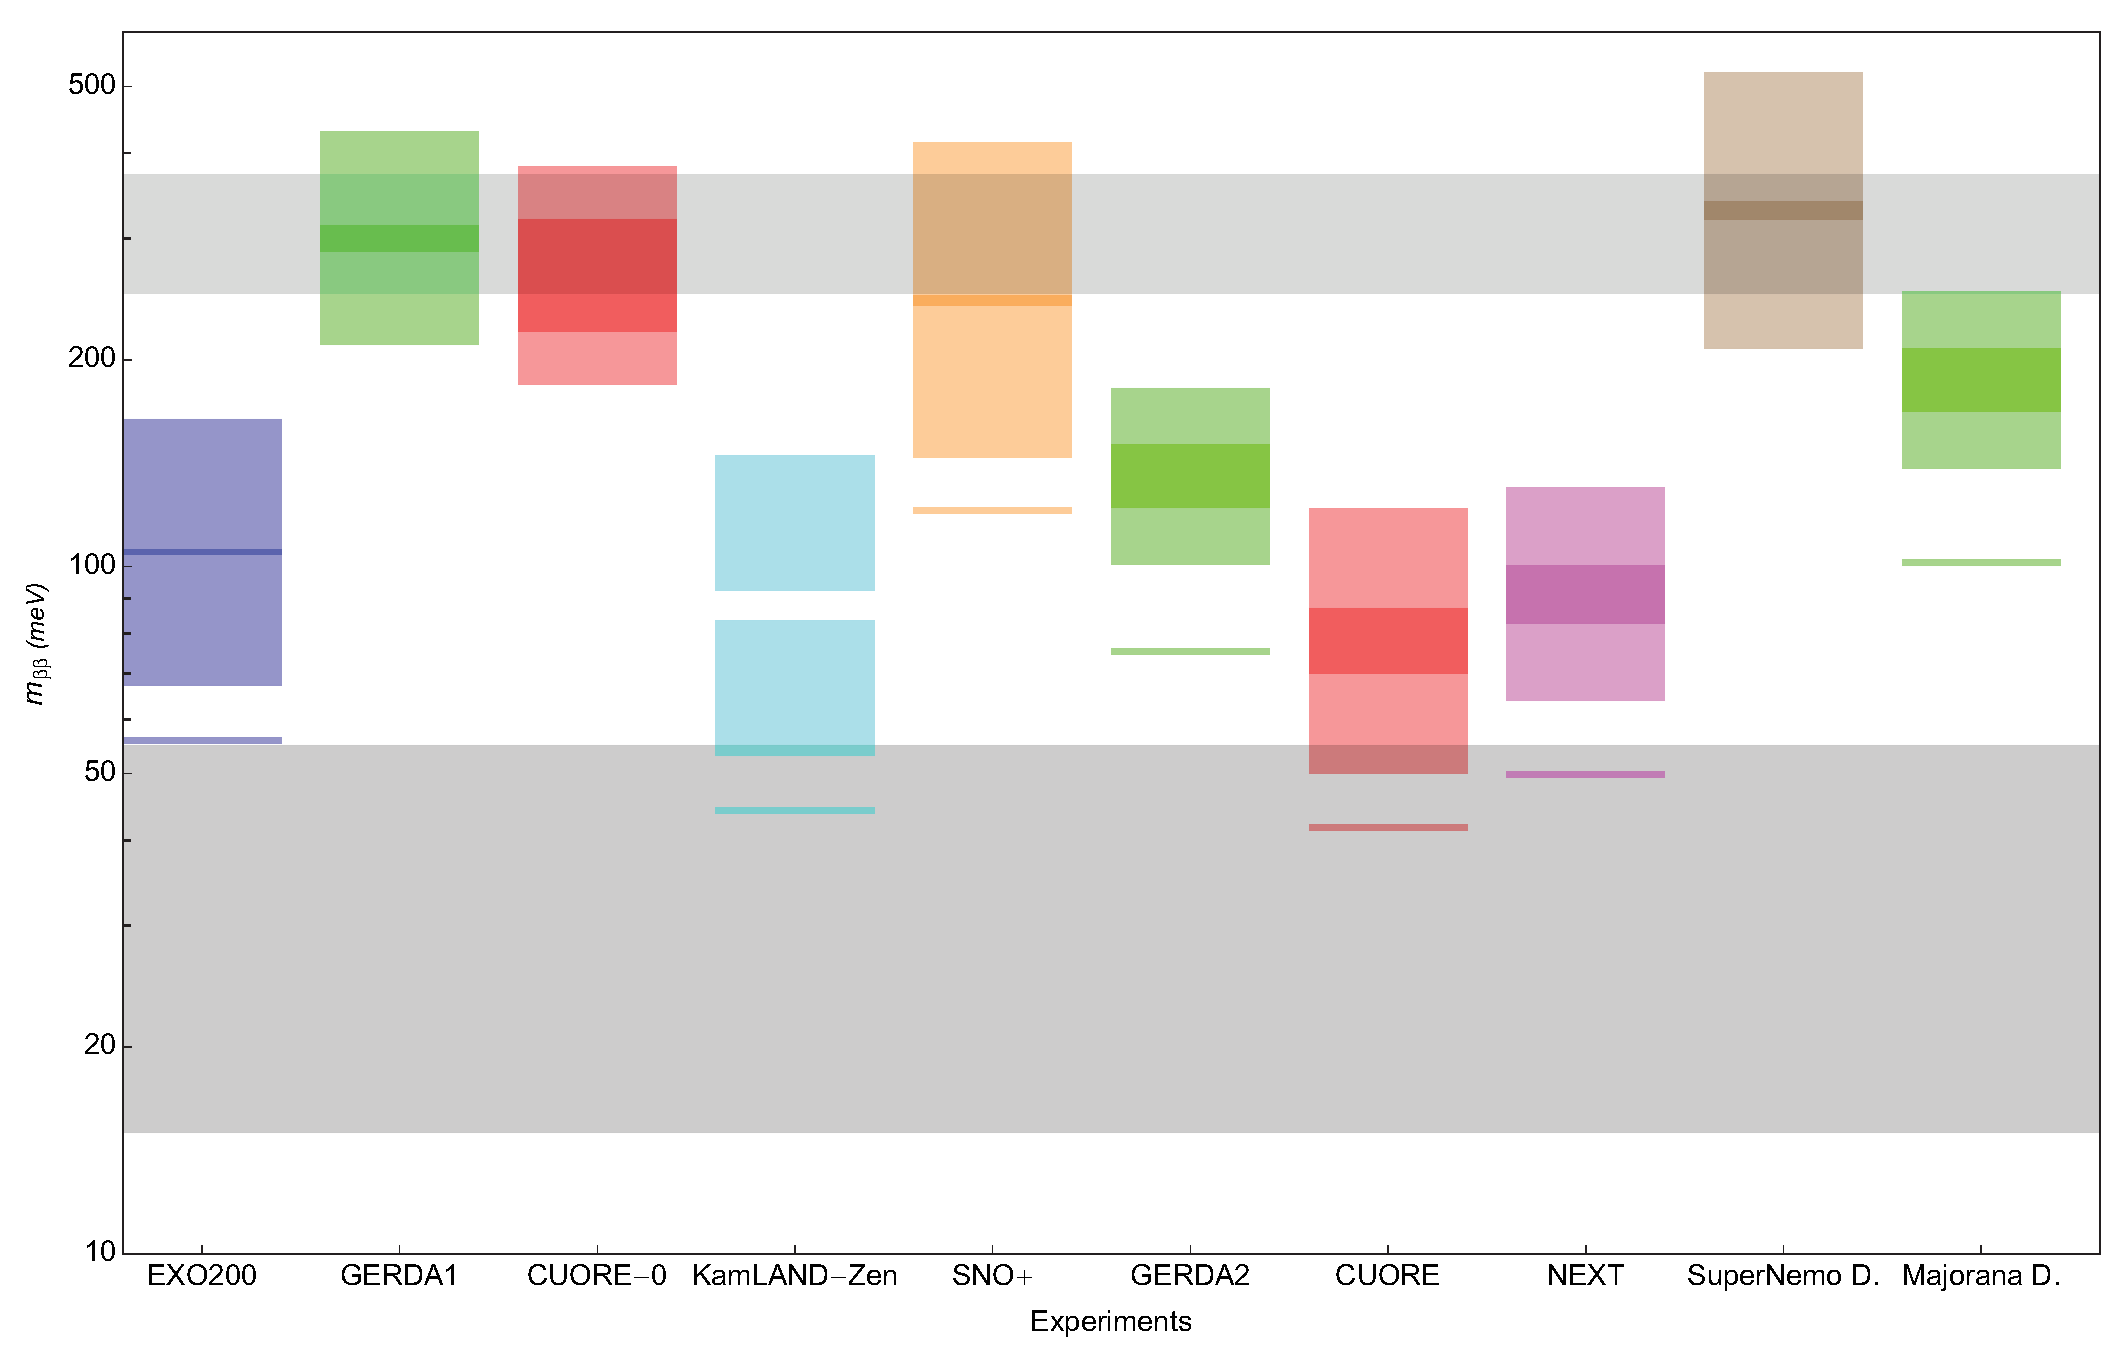
\includegraphics[width=\textwidth]{img/DB_parameters.eps}
\caption{Sensitivity of the different experiments to the neutrino effective mass \mbb\ computed assuming a 5 years exposure, the PMR intervals for the nuclear matrix elements (see sect.~\ref{subsec:nme_pmr}), and for both the optimistic and pessimistic experimental parameters of table~\ref{tab:parameters}. A statistical 90\% CL is computed according to the Feldman-Cousins method \cite{Feldman:1997qc}, assuming a signal region of one FWHM and the corresponding efficiency. For each experiment, the sensitivities for the two experimental parameter sets are drawn as overlapping rectangles. A sensitivity line corresponding to a 10 years exposure, and to the most optimistic NME and experimental parameter set, is also shown. The upper grey region represents the KK claim \cite{Klapdor-Kleingrothaus:2006zcr} while the lower grey region represents the inverted hierarchy region (see fig.~\ref{fig:mbetabetavsmlight}).}
\label{fig:sens-pmr}
\end{figure}


%%%%%
\begin{table}[t!b!]
\caption{Sensitivity of the experiments at 90\% CL after a 5 years exposure, both in terms of half-life \Tonu\ and in terms of neutrino effective mass \mbb . These values are obtained from the optimistic background rate assumptions in tab.~\ref{tab:parameters}. The conversion from \Tonu\ to \mbb\ assumes the central value of the PMR interval for the nuclear matrix elements.}\label{tab:sensitivity}
\begin{center}
%\begin{narrowtabular}{3cm}{lcr}
\begin{tabular}{lcr}
\hline
Experiment & \Tonu\ (years) & \mbb\ (meV) \\ \hline
CUORE-0 	& $8.67\times 10^{24}$ & 203 \\
CUORE 		& $8.86\times 10^{25}$ & 63\\
GERDA-1 	& $4.49\times 10^{25}$ & 252\\
GERDA-2 	& $1.37\times 10^{26}$ & 121\\
EXO200 		& $8.20\times 10^{25}$ & 82\\
NEXT 		& $9.13\times 10^{25}$ & 78\\
KamLAND-Zen 	& $1.32\times 10^{26}$ & 65\\
SNO+ 		& $5.38\times 10^{24}$ & 182\\
SuperNEMO Demonstrator 	& $9.15\times 10^{25}$ & 258\\
MAJORANA Demonstrator	& $7.19\times 10^{25}$ & 258\\
 \hline
%\end{narrowtabular}
\end{tabular}
\end{center}
\end{table}
%%%%%

The first thing to remark from fig.~\ref{fig:sens-pmr} is that the KK claim should be unambiguously solved by several new-generation proposals using different isotopes. If our assumptions are correct, this will certainly be the case for \GE\ (GERDA, MAJORANA), \TE\ (CUORE) and \XE\ (EXO-200, KamLAND-Zen, NEXT), and possibly also for \SE\ (SuperNEMO) and \ND\ (SNO+). Multi-isotope determination of \bbonu\ may therefore become a real possibility within this decade. In this respect, it is important to note that GERDA and MAJORANA are the only experiments among those in fig.~\ref{fig:sens-pmr} using the same isotope of the HM experiment\footnote{Not only: we have seen that GERDA in its first phase re-uses the same detectors as in the HM experiment.}, and should therefore be able to provide the only truly model-independent confirmations of this claim.

On the other hand, several experiments appear to have a very good chance to reach a sensitivity of 100 meV or better, in particular CUORE, KamLAND-Zen, NEXT and EXO-200. In our most optimistic scenario concerning NME values and experimental performances, this target may also be reached by GERDA during its second phase. Given our uncertainties, we cannot predict which, among these 4--5 different experimental proposals, will provide the best \mbb\ sensitivity after a 5 years exposure. To this end, a better knowledge of the actual (as opposed to expected) values for the background rates, of the systematic uncertainties affecting the measurement, and of the NME values would be necessary for all experiments.

From fig.~\ref{fig:sens-pmr}, our expectation is that it will be almost impossible for the new-generation experiments discussed here to discover \bbonu\ after 5 years of exposure if the neutrino mass spectrum is hierarchical ($m_{\rm light}\simeq 0$) rather than degenerate, since essentially no overlap exists between the experimental sensitivities and the 17--52 meV inverted hierarchy region. Not only larger exposures, but also new (better) experimental proposals, would be needed to fully probe this mass region. As mentioned above, we expect experiments using \XE\ (EXO-200, KamLAND-Zen, NEXT) to provide for the first time during this decade a comparable or better sensitivity than \GE\ (GERDA, MAJORANA) and \TE\ (CUORE) experiments, which dominated the field over the past two decades. In perspective, if the low-background expectations of new-generation \XE\ proposals will be confirmed during this decade, \XE\ would be a particularly favorable isotope to use also in the longer term. This is because scalability to isotope masses in the 1-10 ton range are in this case more realistic than with any other isotope. 

\begin{figure}[ht]
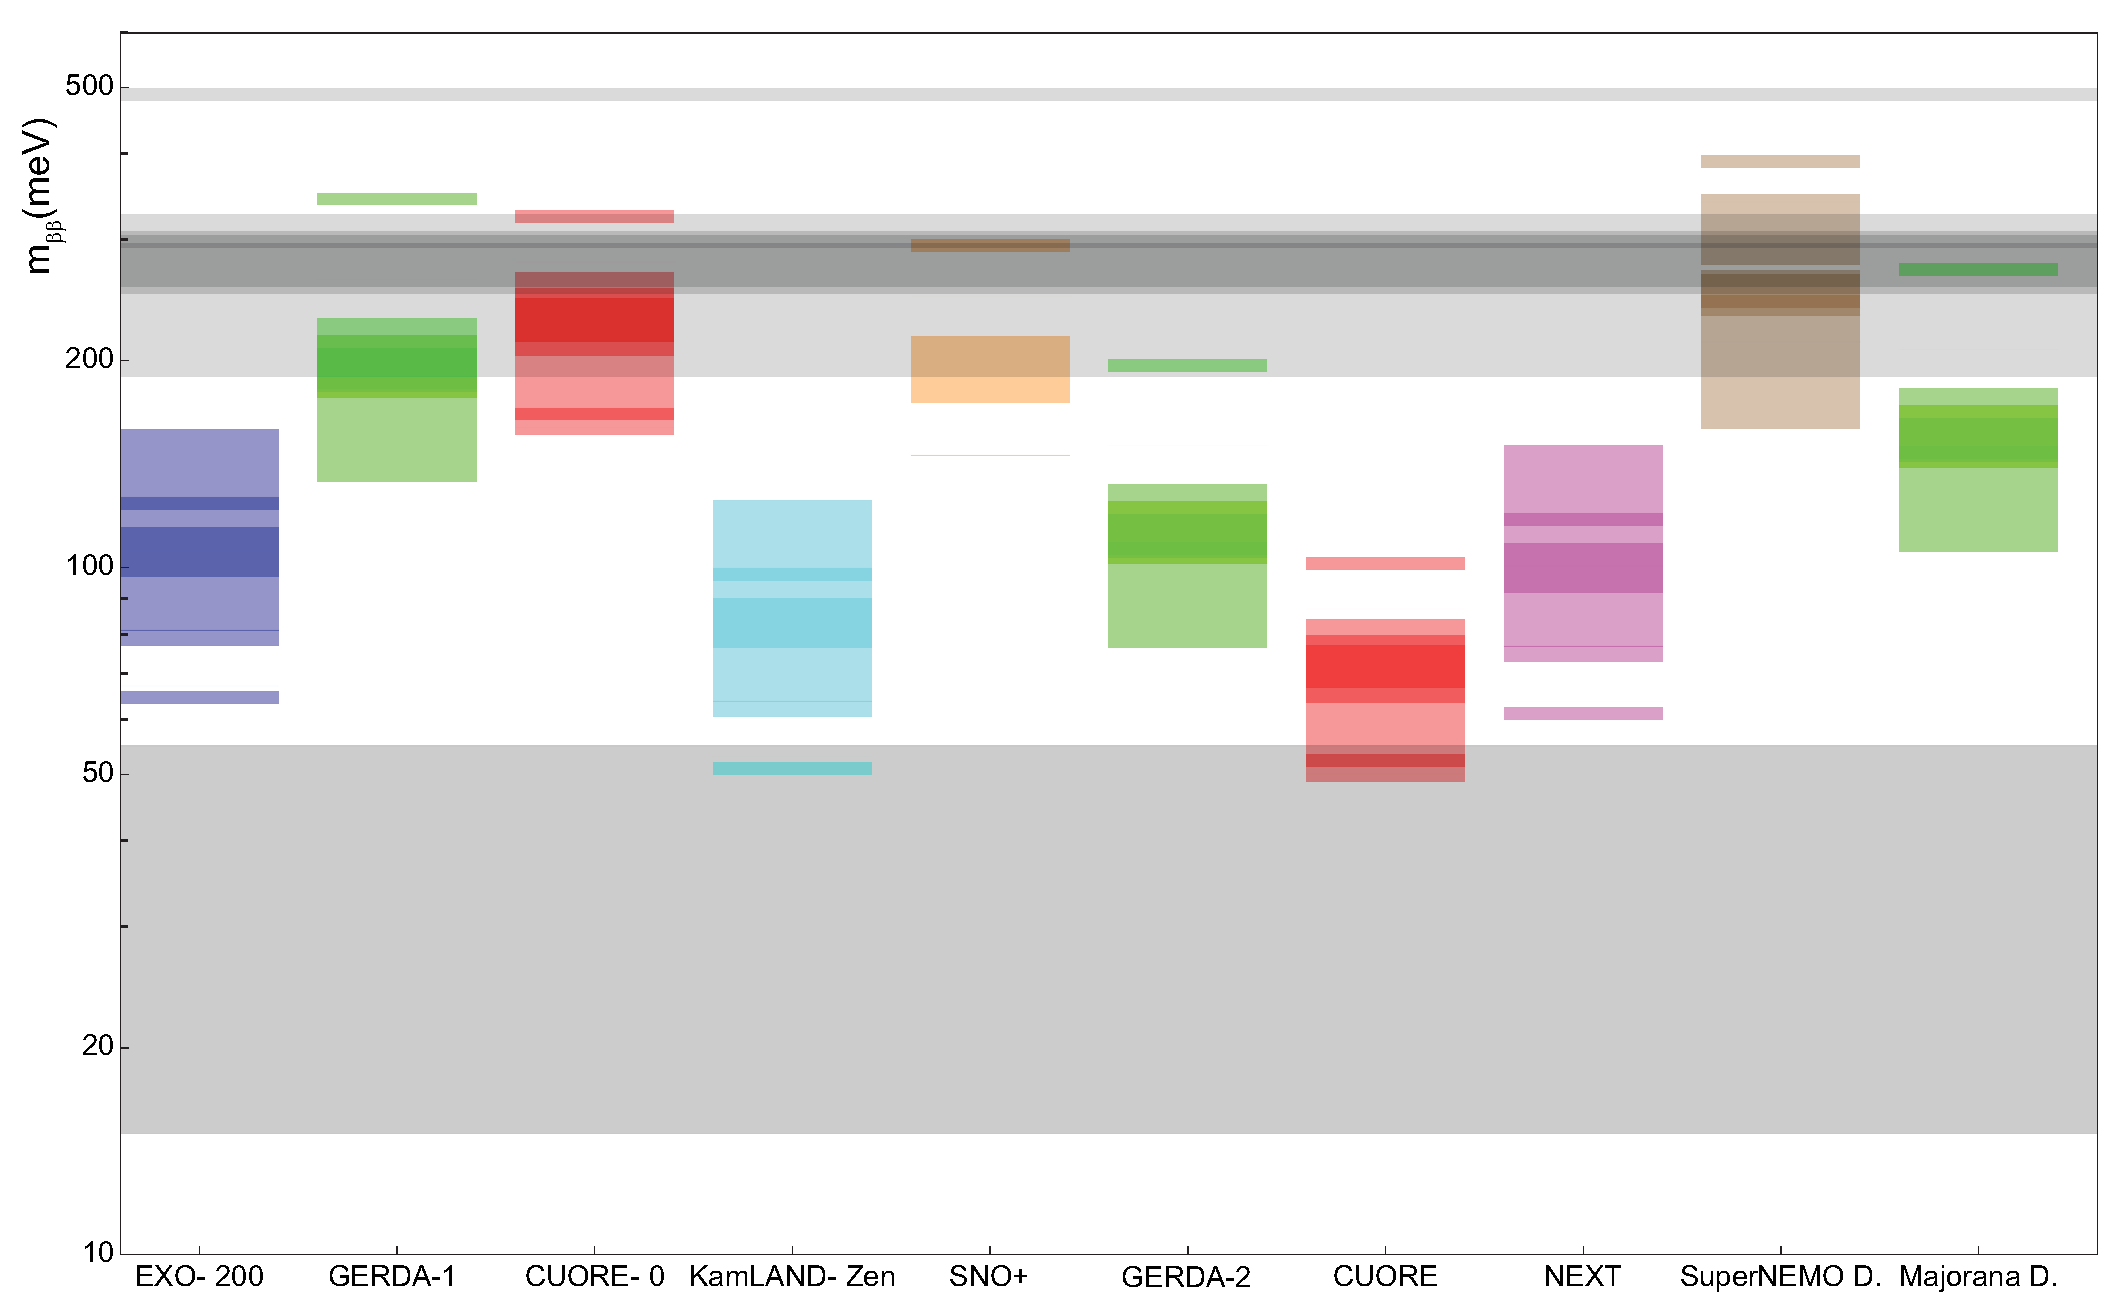
\includegraphics[width=\textwidth]{img/DB_models.eps}
\caption{Sensitivity of the different experiments to the neutrino effective mass \mbb\ computed assuming the optimistic experimental parameters of table~\ref{tab:parameters}. A statistical 90\% CL is computed according to the Feldman-Cousins method \cite{Feldman:1997qc}, assuming a signal region of one FWHM and the corresponding efficiency. Five different frameworks for NME calculations are considered, following reference \cite{Dueck:2011hu}, and are drawn as overlapping rectangles. The upper grey region represents the KK claim \cite{Klapdor-Kleingrothaus:2006zcr} while the lower grey region represents the inverted hierarchy region (see fig.~\ref{fig:mbetabetavsmlight}).}
\label{fig:sens-models}
\end{figure}

Figure~\ref{fig:sens-pmr} represents our main result for the physics case comparison of new-generation \bbonu\ experiments. In this figure, a single, physics-motivated, NME uncertainty band is used for each isotope, following our discussion in sect.~\ref{subsec:nme_pmr}. For completeness, we have also repeated the same exercise for several other NME values or ranges, one for each theoretical framework considered in \cite{Dueck:2011hu}. The result is shown in fig.~\ref{fig:sens-models}. As mentioned above, the spread of the corresponding \mbb\ predictions most likely overestimates the theoretical uncertainty in the \Tonu\ $\to$ \mbb\ sensitivity conversion. For figure clarity, only nuclear theory assumptions are varied in fig.~\ref{fig:sens-models}, while the detector performance parameters are fixed to the most optimistic values of tab.~\ref{tab:parameters}. As can be seen in fig.~\ref{fig:sens-pmr}, our assumed uncertainties in the detector performance parameters would yield \mbb\ sensitivity changes of about the same size as the nuclear theory variations shown in fig.~\ref{fig:sens-models}.
